
\subsection{\ablationadd{Ablation study}}
\label{sec:component_tests}

\relationmemorymark{\stageoneupdate{Full exceeds no-memory \riskall{} by 4.00 points at equal mean core size (Table~\ref{tab:component_main}); the comparison spans batches (Appendix~\ref{app:revision_stage1}).}}

\begin{table}[!tb]
\centering
\renewcommand{\arraystretch}{1.02}
\small

\begin{tabular}{lrr}
\toprule
\bfseries Configuration & \bfseries \riskall{} & \bfseries Comp. \\
\midrule
Stage-1 Full & \stageoneupdate{\tblbest{77.5}} & \stageoneupdate{51.3} \\
\relationmemorymark{\quad No relation memory} & \relationmemorymark{\stageoneupdate{\tblsecond{73.5}}} & \relationmemorymark{\stageoneupdate{51.3}} \\
\quad No critical-pair revisit & \stageoneupdate{56.3} & \stageoneupdate{71.3} \\
\quad Random local window & \stageoneupdate{71.3} & \stageoneupdate{51.3} \\
\midrule
Stage-2 replacement core & \tblbest{75.0} & 51.3 \\
\quad Locked no-replacement & \tblsecond{37.5} & 51.3 \\
\midrule
\multicolumn{3}{c}{\ablationadd{\textbf{Cross-backbone replay: locked $\to$ dynamic}}} \\
\ablationadd{Llama 3.1-8B} & \ablationadd{35.00 $\to$ \tblbest{62.50}} & \ablationadd{51.26} \\
\ablationadd{Qwen3.5-9B} & \ablationadd{33.75 $\to$ \tblbest{57.50}} & \ablationadd{66.55} \\
\ablationadd{Kimi-VL-A3B} & \ablationadd{30.00 $\to$ \tblbest{35.00}} & \ablationadd{51.93} \\
\bottomrule
\end{tabular}
\caption{\stageoneupdate{Ablations (\%) on 80 variants from 20 source SCCs. Stage-1 tests search components on one backbone; core replay covers four backbones.}}
\label{tab:component_main}
\end{table}

\begin{ablationadded}
\paragraph{Shared-evidence replacement.}
Replay fixes evidence proposals and per-case core size. Replacement raises \riskall{} by 5.00--27.50 points on all three further backbones (Table~\ref{tab:component_main}; Appendix~\ref{app:new_core_ablation}). GPT-4o replay yields a 37.50-point gain at equal mean core size (95\% source-SCC paired interval: 12.50--60.00; Appendix~\ref{app:revision_stage2}).

\paragraph{Capacity robustness.}
Matched-size gains persist in all 12 tested model--capacity comparisons (Figure~\ref{fig:capacity_gain}). Appendices~\ref{app:new_selector_control}--\ref{app:new_prefix_analysis} examine selector choice and rollout prefixes.

\begin{figure}[!tb]
\ablationcolor
\centering
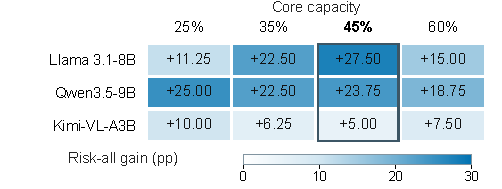
\includegraphics[width=\columnwidth]{figures_ablation_20261011/capacity_gain.pdf}
\caption{Dynamic-minus-locked \riskall{} (pp). Outline: default cap; full results in Appendix~\ref{app:new_core_capacity}.}
\label{fig:capacity_gain}
\end{figure}
\end{ablationadded}

\subsection{Cost and sensitive analysis}
\label{sec:cost_analysis}

\begin{table}[!tb]
\centering
\renewcommand{\arraystretch}{1.02}
\small

\begin{tabular}{lrrrr}
\toprule
  & \multicolumn{2}{c}{\bfseries \riskall{} (\%)} &   &   \\
\bfseries Method & \bfseries GPT-4o & \bfseries \revvalue{Pro}{Gemini} & \bfseries Calls & \bfseries Tokens \\
\midrule
One-shot & 25.0 & \tblbest{100.0} & \tblbest{1.0} & \tblbest{23.5}K \\
LEA & \tblsecond{41.7} & 83.3 & \tblsecond{16.9} & \tblsecond{63.7}K \\
\rowcolor{TableFocus}
\textbf{\samcgs{}} & \tblbest{83.3} & \tblsecond{91.7} & 56.5 & 203.4K \\
\bottomrule
\end{tabular}
\caption{\revreplace{Contemporaneous cost--performance comparison on 12 sources, two models, and three methods (72 runs). \riskall{} uses strict scoring. Calls and tokens are averaged across models and include observed recovery work.}{Cost--performance: 12 sources, 72 runs, GPT-4o/Gemini 2.5 Pro. Strict \riskall{} ($\uparrow$); model-averaged calls/tokens ($\downarrow$) include recovery. Bold/underline: best/second-best per column. Shading: \samcgs{}.}}
\label{tab:cost_main}
\end{table}

Table~\ref{tab:cost_main} reports inference costs and endpoint retention. \samcgs{} uses about 3.2 times as many tokens as LEA, with \riskall{} gains of 41.7 percentage points on GPT-4o (95\% CI: 8.3--75.0) and 8.3 on Gemini 2.5 Pro (\mbox{$-16.7$--33.3}). One-shot performs best on Gemini in this sample. Three invalid GPT-4o One-shot outputs remain in the denominator. Concurrent rollouts can reduce wall-clock time without reducing token use; Appendix~\ref{app:revision_cost} details the parallel-time model and recovery accounting.

On four prespecified sources, varying the relation-prior bonus multiplier by $\pm20\%$ does not reduce final \riskall{} but changes \rootthree{}. This single-coefficient check does not establish robustness to other priors or thresholds (Appendix~\ref{app:revision_prior}).



\subsection{Expert evidence and unmodified sources}
\label{sec:expert_main}

\revadd{Experts select a \emph{minimal evidence set} $M$, the fewest records supporting their risk judgment, and a broader \emph{repair-material set} $R$ with context needed to understand and repair the risk. We assess 24 injected variants and 18 unmodified sources. For the latter, a third expert independently adjudicates under fully blinded conditions whenever the first two disagree on risk existence or either reports confidence below 3/5.}

\revadd{On the 24 variants (14 sources), source-weighted minimal-evidence recall is 90.8\% for GPT-4o \samcgs{} versus 65.4\% for LEA, and 88.5\% versus 86.3\% for Gemini 2.5 Pro. Repair-reference precision rises from 66.5\% to 85.0\% and from 71.8\% to 88.4\%, respectively (confidence intervals in Appendix~\ref{app:expert_extension}).}

\revadd{Among the unmodified sources, experts identify 15 risk and three no-risk cases. \samcgs{} flags all 15 risk cases with both models, matching expert judgments on 18/18 (100.0\%) with GPT-4o and 15/18 (83.3\%) with Gemini 2.5 Pro. All errors are false alarms. These results extend evaluation beyond controlled injection, with backbone-dependent no-risk recognition.
}
